% Capítulo 2 - vFinal 1.0 - 05/07/2018
\chapter{Conceitos Relacionados}
\label{cap:cap2}

Este capítulo aborda os conceitos e técnicas que proporcionam a compreensão dos capítulos a seguir. Na Seção \ref{cap2:iot}, apresento a visão geral sobre Redes IoT e dispositivos que compõe o alvo das iniciativas propostas. A Seção \ref{cap2:energyDriven} introduz o conceito da computação dirigida aos fatores energéticos, tema originador do trabalho.  Por sua vez, na Seção \ref{cap2:throttling} encontram-se os conceitos ligados ao padrão throttling, seus objetivos e aplicação. A intenção de uso de um modelo taxonômico esta fundamentada na Seção \ref{cap2:taxonomia}. Ao fim, na Seção \ref{cap2:consideracoesFinais} estão descritas as considerações ao capítulo.


\section{Internet das Coisas}
\label{cap2:iot}

O termo IoT - Internet das Coisas (\textit{Internet of Things}), foi proposto inicialmente por \citeauthor{ashton1999internet} (\citeyear{ashton1999internet}), e descreve a capacidade de objetos físicos estarem interconectados por meio da internet, viabilizando seus processos de coleta e compartilhamento de dados. Atualmente, a quantidade de dispositivos interconectados cresce diariamente em números impressionantes \cite{lund2014worldwide} uma breve observação da vida diária comprova que nunca tivemos tantos dispositivos inteligentes ao nosso redor, com diversas projeções sendo criadas a respeito da quantidade de elementos interconectados.

Possibilitando a comunicação entre dispositivos,  redes inteligentes podem ser controladas remotamente e automatizadas para realizar tarefas específicas. Essas características favorecem uma variedade de aplicações, incluindo monitoramento, gerenciamento de recursos, saúde digital, cidades inteligentes, agricultura de precisão, e o desenvolvimento de novas aplicações \cite{miorandi2012internet, asghari_internet_2019}.

No entanto, com essa capacidade aprimorada, novos desafios são encontrados à medida que novas aplicações aproveitam suas potencialidades, resultando em soluções mais amplas e aprimoradas a passo que crescem em complexidade. Por exemplo, o aumento do numero de dispositivos interconectados exige uma abordagem mais sofisticada para gerenciamento e segurança em decorrência da massiva quantidade de dados gerados e compartilhados, em paralelo, a interoperabilidade dos sistemas atingem maior importância a medida que o ecossistema das Redes IoT se expande. 

Na revisão proposta em \cite{asghari_internet_2019}, podemos caracterizar os elementos presentes na \acs{IoT}, e, entre outros fatores, de acordo com as seguintes capacidades:

\begin{enumerate}
	%self-adapting
	\item Capacidade de auto-adaptação: Dispositivos e sistemas IoT precisam ser capazes de dinamicamente adaptar-se mudando seu contexto e tomando ações motivadas nas suas condições de operação e contexto de uso. Considerando um sistema de monitoramento de ambientes com câmeras, estas podem adaptar seu modo de operação (com e sem iluminação suficiente) baseando se está de dia ou noite \cite{doumenis_lightweight_2022}. 
	
	%self-configure
	\item Capacidade de auto-configuração: Dispositivos carregam a capacidade de auto configuração, permitindo que dispositivos atuem em conjunto para prover alguma funcionalidade. Estes podem configurar a si mesmo (associado a infraestrutura provida).
	
	%Interoperability
	\item interoperabilidade entre protocolos: Dispositivos IoT podem suportar diversos protocolos de comunicação com outros elementos e infraestrutura.
	
	%Context-awareness
	\item Consciência de Contexto: Uma vez imerso no meio físico, dispositivos podem adquirir conhecimento a respeito das características que o cerca. As decisões tomadas posteriormente podem levar em consideração esses aspectos \cite{yang2014health}.
\end{enumerate}

Neste quesito, os aspectos ligados aos fatores energéticos também se destacam, sobretudo quando estão relacionados aos desafios de manter dispositivos operando eficientemente e de maneira sustentável \cite{albreem_green_2017}. Questões ligadas a eficiência energética, autonomia e a busca de fontes alternativas de suprimento energético bem como a capacidade dos dispositivos em lidar com tais fatores são pontos fundamentais a se pensar. 

Restrições energéticas permanecem como um dos principais temas, desafio que afeta a performance e disponibilidade de elementos nas redes IoT. Atualmente, as soluções mais promissoras para tal são os esforços na gerencia de energia \cite{singh_survey_2020}. Em alguns cenários, a solução mais adequada para estas questões passa pela ação de coletar energia do meio onde o dispositivo esta inserido. Segundo \cite{kansal_power_2007}, um \ac{EHS} ou Sistema de Coleta Energética é o dado sistema complexo capaz de captar energia do ambiente que se encontram convertendo para seu uso.

Desde modo, dispositivos encontrados em tal cenário carregam em suas características fundamentais a necessidade de lidar com os aspectos energéticos, como proposto por \citeauthor{kansal_power_2007} (\citeyear{kansal_power_2007}). Sobretudo com a capacidade de coleta energética, algumas estratégias podem ser tomadas com base nas características embarcadas nos dispositivos, pois em tal cenário precisam ser projetados com a capacidade de autoadaptação, permitindo ajustar-se dinamicamente em acordo com as condições encontradas, demandas operacionais e oferta energética. A consciência de contexto aqui permite a eles compreender e responder às mudanças no ambiente circundante, adaptando-se ou reconfigurando-se proativamente para operar adequadamente frente as condições encontradas. Essas capacidades combinadas com seu sistema de coleta de energia habilita que dispositivos IoT possam gerenciar seus aspectos energéticos de maneira inteligente e responsiva, otimizando seu desempenho enquanto minimizam o consumo de energia buscando perpetuar-se disponível, desde que projetado para tal, contribuindo sobretudo para eficiência geral dos sistemas IoT.



%desafios energéticos para IoT

%areas de solução

\section{\textit{Energy-Driven Computing}}
\label{cap2:energyDriven}

Um sistema dirigido à energia (\textit{Energy-Driven}) é todo aquele que os fatores energéticos intrínsecos a ele são tratados como primários, desde concepção, gerenciamento e sua operação \cite{merrett_energy-driven_2017}. Computação dirigida a estes fatores, ditos energéticos, deve considerar fundamentalmente a disponibilidade energética pois precisam carregar a capacidade de adaptação as dinâmicas de captação de energia. Este paradigma tem como objetivo evidenciar as características energéticas, em potencial a respeito de dispositivos que por quaisquer motivos, não podem estar conectados diretamente em uma infraestrutura capaz de fornecer energia virtualmente ilimitada. 

Para tal, caso necessário, dispositivos podem operar coletando recursos disponíveis no ambiente. Coleta de energia refere-se a capacidade de um dispositivo em capturar e converter recursos energéticos do meio e converte-los de modo a prolongar sua vida útil mitigando um cenário de escassez energética \cite{sudevalayam_energy_2011}. 

Ainda, no trabalho de \citeauthor{sliper_energy-driven_2020} (\citeyear{sliper_energy-driven_2020}) é importante destacar como os mecanismos de coleta energética e sua dinâmica são dispostos. É proposto uma organização em três categorias distintas: Neutra-Energética \ac{EN}, Neutra-Força ou Neutra em Consumo \ac{PNO} e por fim, Operações Intermitentes.

\subsection{Operação \textit{Neutra-Energética}}
Uma operação neutra-energética cobre as dinâmicas dos sistemas com coleta de energia do ambiente por meio de um \textit{buffer}, uma bateria recarregável ou super capacitor capaz de armazenar parte da energia coletada \cite{kansal_power_2007}. Este recurso se encontra disposto entre a entrada energética e sua demanda, atuando secundariamente quando a energia disponibilizada não seria suficiente para manter seus critérios de qualidade de serviço \textit{QoS}.

Apesar de inicialmente ser previsto um cenário de uso onde apenas a fonte energética e o dispositivo estivessem presentes, é comum o fato dos mecanismos que buscam esse tipo de operação recorrer a presença deste componente intermediário capaz de armazenar energia e disponibiliza-la para uso. Sendo assim, na Figura \ref{fig:cap2harveststoreuse} temos a visão geral em blocos de um subsistema responsável pelos recursos energéticos.

\begin{figure}[H]
	\centering
	\caption{Diagrama de blocos subsistema energético para operação neutro-energética.}
	\label{fig:cap2harveststoreuse}
	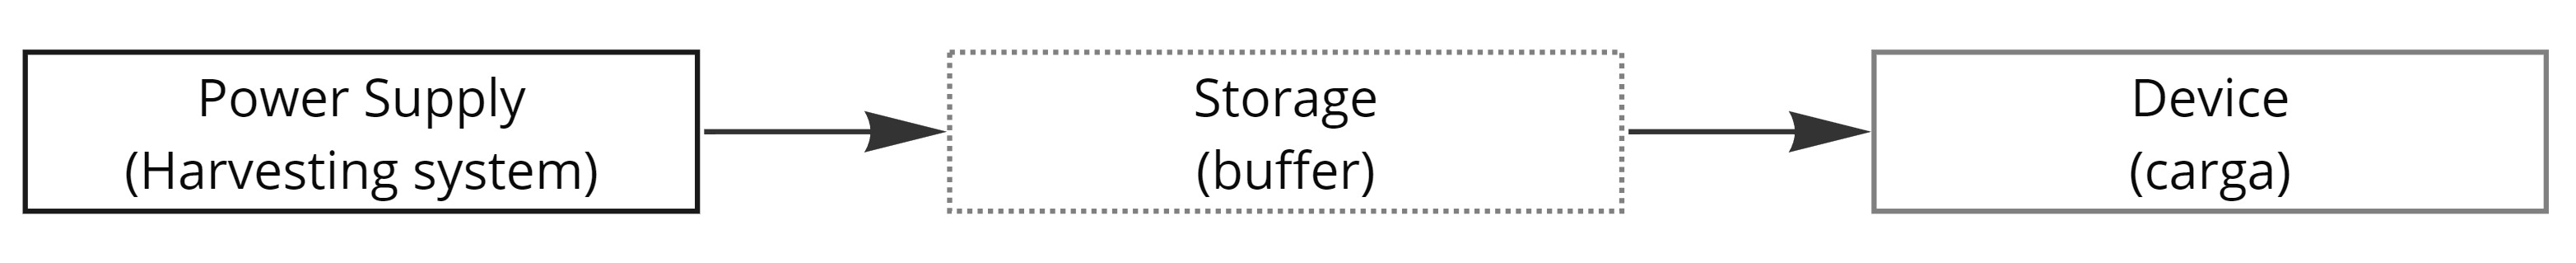
\includegraphics[width=0.7\linewidth]{Imagens/cap2/cap2harvest_store_use}	
	
	Fonte: adaptado de \citeauthor{sudevalayam_energy_2011} (\citeyear{sudevalayam_energy_2011} )
\end{figure}

A visão do cenário acima proporciona ao node a capacidade de manter seus níveis de operação, abstraindo em algum nível as variações de energia coletada. Pois seja $P_{s}(t)$ a entrada energética em dado momento e  $P_{c}(t)$ a energia consumida nos ciclos de carga, é possível encontrar a dinâmica apresentada na Figura \ref{fig:cap2energyneutraloperation}, em momento de abundancia energética o node pode armazenar a energia que supera a quantidade necessária para sua operação em decorrência de que em momentos de escassez, possa fazer uso dessa energia suplementando sua necessidade. 


Operações neutro-energéticas carregam dois princípios que são apresentados no trabalho seminal \cite{kansal_power_2007}: Manter-se operacional mesmo em cenários onde a quantidade de energia coletada fosse durante muito tempo, inferior ao necessário e como garantir que, encontrado em um ambiente de coleta seja possível obter performance esperada tolerando variações da energia coletada. 

\begin{figure}[H]
	\centering
	\caption{Dinâmicas de operação com coleta de energia} \label{fig:dinamicas}
	\begin{subfigure}{0.49\textwidth}
		\caption{Operação com buffer intermediário.}
		\label{fig:cap2energyneutraloperation}
		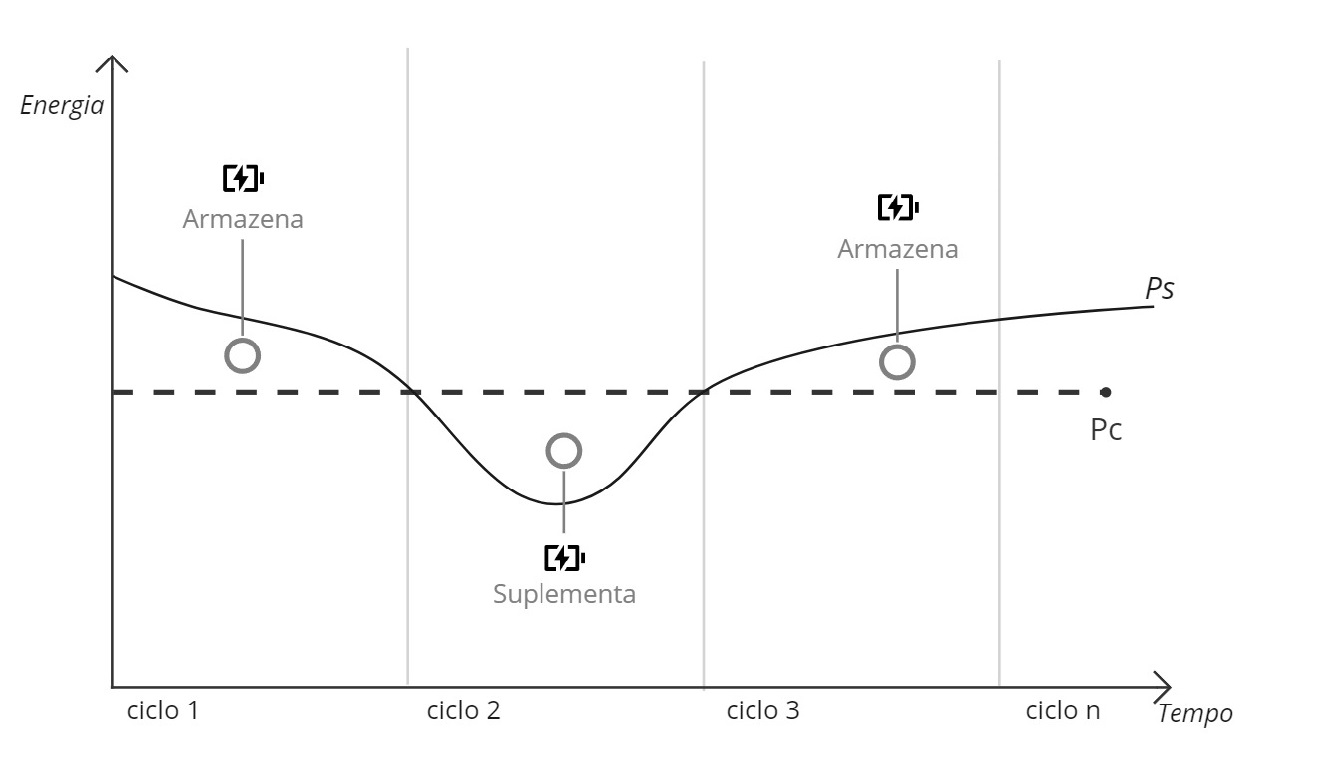
\includegraphics[width=\linewidth]{Imagens/cap2/cap2energyneutraloperation.jpg}	
	\end{subfigure}%
	\hspace*{\fill}  
	\begin{subfigure}{0.49\textwidth}
		\caption{Operação Power-Neutral.}
		\label{fig:cap2powerneutraloperation}
		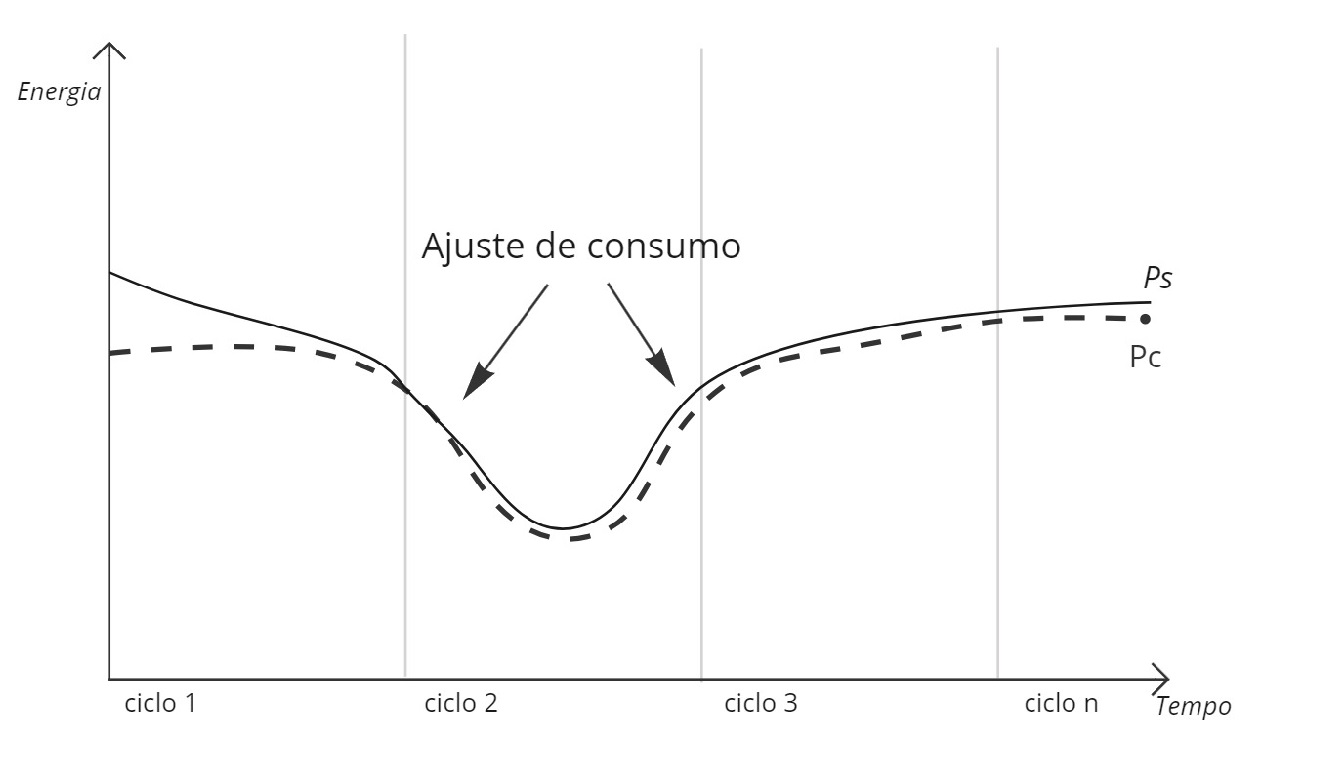
\includegraphics[width=\linewidth]{Imagens/cap2/cap2powerneutraloperation.jpg}
	\end{subfigure}%
	\hspace*{\fill}   
	
	Fonte: elaborado pelo autor.
\end{figure}

Sendo assim, uma operação neutro-energética implica em manter sua a performance durante os ciclos de trabalho garantindo que o node não sofra por esgotamento energético. Busca-se perpetuar sua operação mediante uso da reserva energética ou adaptação motivada a expectativa de recurso futuro \cite{sudevalayam_energy_2011}. Desta forma, o dispositivo favorecido pode prolongar sua operação mesmo em decorrência da indisponibilidade ou insuficiência de fonte energética.

É importante destacar que este modo de operação serviu como base para diversos avanços em computação dirigida a energia sobretudo em redes constituídas tipicamente com sensores embarcados, autônomos e distribuídos espacialmente, \acf{WSN}. Além disso, os conceitos de operação-neutra e a teoria de coleta energética foram fundamentais para o que posteriormente foi detalhado em referencia ao seminal \cite{merrett_energy-driven_2017}, introdutório ao modelo \acf{PNO}.



\subsection{Operação \textit{Power-Neutral}}
A capacidade de um dispositivo em coletar energia do ambiente apresenta diversos desafios, especialmente em relação ao processo de coleta, transformação e uso, bem como à previsibilidade da oferta de energia. A abordagem ilustrada na Figura \ref{fig:cap2harveststoreuse} é típica de um sistema que utiliza um buffer intermediário, com o objetivo de operar semelhante a um sistema tipicamente alimentado por baterias, onde as condições energéticas são resumidas apenas pela condição da reserva energética disponível. No entanto, em muitos casos, os componentes adicionais necessários para garantir essas características aumentam custos, volume e complexidade, podendo resultar em comportamento não confiável se mal projetados.

De acordo com \citeauthor{merrett_energy-driven_2017}(\citeyear{merrett_energy-driven_2017}), os esforços para projetar sistemas com capacidade de coleta de energia devem agora considerar casos onde não é possível incluir um componente de armazenamento energético intermediário. Portanto, os sistemas nessas condições devem buscar o modo intermitente ou mesmo \textit{Power-Neutral}, conforme ilustrado na Figura \ref{fig:cap2powerneutraloperation}.

A Operação \textit{Power-Neutral} envolve adaptar o consumo de energia do dispositivo para manter sua operação de acordo com os recursos disponíveis, minimizando ou até mesmo eliminando a necessidade de armazenamento intermediário de energia \cite{sliper_energy-driven_2020}. No entanto, é importante observar que, se a energia coletada for inferior ao mínimo necessário, o dispositivo entrará em um estado de esgotamento, podendo hibernar caso caracterizado por uma abordagem intermitente \cite{merrett_energy-driven_2017}.



\section{\textit{Throttling}: Padrão de Comportamento em Ambientes Distribuídos}
\label{cap2:throttling}

Como ponto de partida, é preciso destacar a importância da adoção dos ditos padrões \textit{patterns}, especialmente aplicados em sistemas distribuídos. Tais soluções carregam aspectos intrínsecos à experiencia adquirida mediante a recorrência de soluções frente à heterogeneidade de problemas que corrigem, formando o conjunto de atuação onde um ou mais padrões de solução emergem como resposta. Endossado pelo trabalho de \citeauthor{burns_designing_nodate} (\citeyear{burns_designing_nodate}) e no cenário de computação distribuída, é observado que apesar da diversidade de possibilidades para um sistema qualquer, a maneira como é concebido, desenvolvido e por consequência os problemas encontrados sobretudo quanto  aspectos não funcionais como escalabilidade, confiabilidade ou disponibilidade são notavelmente recorrentes e semelhantes. 

O proposito de adotar o padrão Throttling é fazer com que dado sistema alvo mantenha seus níveis de consumo abaixo de um determinado termo, limiar. Assim, conservando seus recursos disponíveis que de outra forma seriam disponibilizados para solicitantes excessivamente demandantes. Além de proteger-se do comportamento inadequado dos agentes envolvidos, é preciso ter em mente que eventualmente um sistema pode encontrar-se tendo de lidar com picos de operações, cenário propício a falhas ou até mesmo interrupção integral do serviços. 

Ambientes IoT representam um domínio onde esse padrão pode ser bastante necessário dado a dinâmica de dispositivos desconhecidos e novos sistemas que podem ser adicionados a um ambiente. Throttling pode ser implementado segundo algumas estratégias elencadas por \citeauthor{martinekuan_throttling_nodate} (\citeyear{martinekuan_throttling_nodate}):

\begin{itemize}
	\item Rejeitando requisições de um agente excessivamente solicitante.
	\item Desabilitando ou degradando componentes ligados a operações menos essenciais. 
	\item Estabelecendo níveis de prioridade para os agentes solicitantes, onde requisições de níveis menos prioritários podem ser suspensas ou limitadas em detrimento de outra com mais privilégio, durante algum tempo, conforme Figura \ref{fig:cap2throttlingexample}.
\end{itemize}

\begin{figure}[H]
	\centering
	\caption{Throttling pode ser aplicado uma vez estabelecidos critérios de prioridade de operações}
	\label{fig:cap2throttlingexample}
	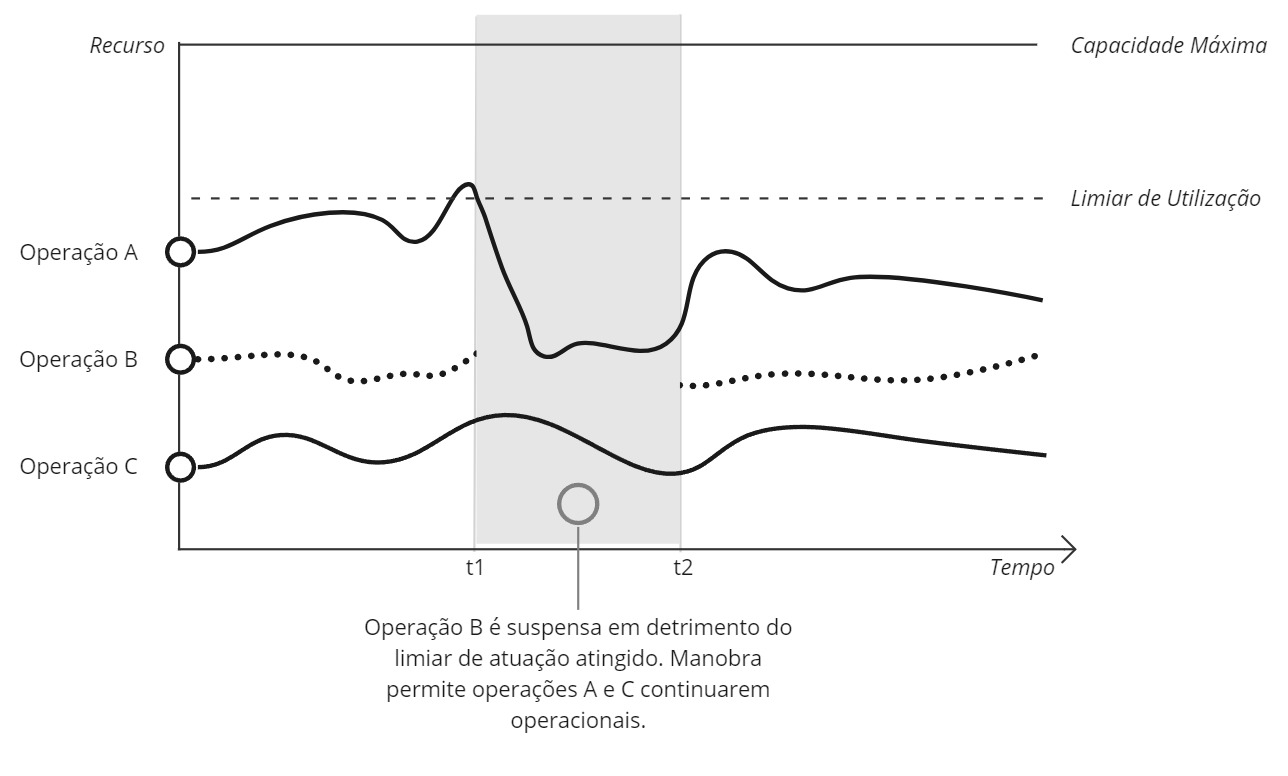
\includegraphics[width=0.7\linewidth]{Imagens/cap2/cap2throttlingexample}	
	
	Fonte: adaptado de \citeauthor{martinekuan_throttling_nodate} (\citeyear{martinekuan_throttling_nodate})
\end{figure}

\subsection{Considerações}
Assim como outros padrões aplicados a sistemas distribuídos, existem uma série de considerações a serem tomadas mediante a decisão de implementar um mecanismo de throttling, \cite{martinekuan_throttling_nodate} aponta alguns tópicos que possibilitam a análise de conformidade face aos problemas e necessidades ao adotar o padrão.  

Utilizar mecanismos de throttling passam por decisões arquiteturais de como o dispositivo vai se comportar. Por isso, deve-se levantar primariamente seu uso nos estágios iniciais de concepção do dispositivo ou sistema.

Um vez estabelecido, caso limiar de atuação seja atingido, os mecanismo de throttling deve ser acionado em conformidade, e uma vez restabelecido ao seu estado regular de atuação, permitir o retorno as capacidades do dispositivo.

É interessante padronizar os retornos dados as solicitações negadas ativamente pela ação do throttling, dando condições do agente solicitante em tomar a melhor decisão entre refazer a solicitação ou aguardar momento oportuno.

Dispositivos capazes de adaptar-se mediante quaisquer fatores devem ter seu comportamento refletido no mecanismo de throttling, preferencialmente em tempo de execução. Eventualmente um cenário onde amparado por uma condição do dispositivo seria tolerado pode não ser mais, o movimento inverso também é valido, condições não toleradas podem passar a ser, mediante evento motivador. 

\section{Taxonomia}
\label{cap2:taxonomia}

Taxonomia refere-se a um sistema de classificação e organização. Seu modelo consiste em sistematicamente apresentar os elementos de um campo de estudo, categorizados e por conseguinte classificados de modo a apresentar os elementos dispostos em estrutura adequada.

O mapeamento sistemático apresentado por \citeauthor{usman_taxonomies_2017} (\citeyear{usman_taxonomies_2017}), trata dos métodos e da aplicação de taxonomias em campos da engenharia de software. O procedimento classificação define como as instâncias de um tema podem ser atribuídos a classes ou categorias. Para uma taxonomia, tais elementos podem estar relacionados e dependentes entre si. Por sua vez, é possível classificar de duas maneiras: Quantitativamente, onde os procedimentos de classificação são baseados em escalas numéricas ou Qualitativa onde uma escala nominal que expresse a categoria será utilizada. Sua estrutura, poderá ser dividida em quatro visões de descobrimento do conhecimento \cite{kwasnik_role_nodate}.

\textbf{Hierárquica}, aqui a taxonomia é estruturada como uma única classe superior (superclasse) que abrange suas subclasses e sequencialmente as possíveis extensões destas, formando um encadeamento hierárquico entre os elementos desde o originário até os derradeiros derivados. Este modelo procura garantir a exclusão mutua entre os envolvidos além do aspecto de relacionamento hereditário, por isso não é recomendado em situações onde uma pesquisa precisa incluir múltiplos e diversos critérios de diferenciação. Por fim, o autor considera que para esta representação é mandatório bom conhecimento sobre o assunto a ser classificado., pois suas classes e critérios de separação precisam ser conhecidos desde o inicio.

\textbf{Árvore} similar ao modelo hierárquico, todavia em uma estrutura árvore não existe um relacionamento do tipo herança. Aqui, o tipo de classificação que busca-se é a relação causa-efeito, processo-produto ou parte-todo. Pode-se usar a estrutura arvore para mostrar a decomposição de um tema em seus aspectos. Por exemplo, a representação em árvore parte-todo do relacionamento entre um país, seus estados e por fim, municípios. Estruturas árvores e hierárquicas compartilham das mesmas limitações.

\textbf{Paradigma}, conduz a taxonomia para a capacidade de um relacionamento bi-direcional entre as classes estas, por sua vez, podem ser descritas pela combinação de dois atributos. Uma proposta de visualização para taxonomias desse tipo é a capacidade de expressar-se com matrizes bi-dimensionais cujo seus vértices apresentam os atributos de interesse.

\textbf{Facetada}, esta estrutura taxonômica permite observar os assuntos classificados sob múltiplas perspectivas (facetas). O indicador fundamental em utilizar uma análise facetada é a necessidade de visualizar mais de uma perspectiva de uma entidade complexa. Cada faceta é independente e pode ter suas próprias classes, permitindo a evolução de cada uma dentro da sua perspectiva. Análise facetada é adequada para campos de conhecimento relativamente novos em constante evolução, dado que não é necessário ter o completo conhecimento do objeto de estudo. Em todo caso, pode ser desafiador encontrar o conjunto inicial de facetas para a taxonomia de modo que sejam independentes e sem aparente relacionamento significativo entre as facetas.

Em \cite{smite_empirically_2014}, o autor indica três mecanismos como validadores de uma taxonomia: a demonstração ortogonal de perpendicularidade e dimensões das classes é demonstrada; análise de desempenho (\textit{Benchmarking}), em que a taxonomia pode ser comparada com outros esquemas de classificação similares; e, por fim, a demonstração de utilidade, validada por estudo de caso ou experimentação.

O entendimento sobre qual visão utilizada para construção de uma taxonomia é crucial, pois impacta diretamente na sobre a maneira como representar classes e interações. Quanto à aplicação prática para Engenharia de Software, ao adotar o uso de uma taxonomia proporciona os agentes facilitadores para atividades de classificar e organizar o conhecimento de uma determinada área \cite{usman_taxonomies_2017}, auxiliando no desdobramento do objeto de estudo, elucidação e identificação de oportunidades e trabalhos futuros.

\section{Considerações Finais}
 \label{cap2:consideracoesFinais}
 
 Neste capítulo foram apresentado os conceitos relacionados que indicam o apoio teórico necessário para a construção do trabalho. Assim, a Seção \ref{cap2:iot} apresenta uma introdução à IoT em destaque para relação com a problemática das restrições energéticas e os mecanismos de coleta energética. A seguir, na Seção \ref{cap2:energyDriven} são descritos os principais modos de operação para computação dirigida a energia \textit{Energy-Drive Computing}. Posteriormente, Seção \ref{cap2:throttling} trás o agente motivador para uso de padrões utilizados em sistemas distribuídos, em especifico Throttling, como um artefato adequado para controle de comportamento dos dispositivos mediante mudança de contexto. Por último, a Seção \ref{cap2:Taxonomia} destacou os propósitos de uma taxonomia e explicou como essa abordagem pode ser útil para organizar um conhecimento e identificar áreas de pesquisa importantes.
